\section{Methods}\label{sec:methods}
\subsection{Data} \label{subsec:data}

\subsubsection{Automated plankton imagers}

The models were applied to two sets of images from different imaging hardware (figure \ref{fig:plankton-img}). The first, PlanktoScope, is an automated quantitative plankton imaging system which can be built with a Raspberry Pi and standard parts \cite{pollina2022:planktoscope}. The imaging is based on a flow-through system, where the sample is pumped through a flat glass capillary and imaged, stopping the flow for every image to avoid distortion. The size range of the imaged objects is dependent on the camera quality and capillary width, and was in our setup constrained to objects between 40-200 µm. Although the imaging itself is automated, using the PlanktoScope is dependent on manually sampling for material, e.g., field sampling with a plankton net. The samples are backlit, resulting in images with a light background.

The other hardware is a Continuous Particle Imaging Classification System (CPICS), which is an in-situ plankton imaging system (\hyperlink{https://www.coastaloceanvision.com/cpics}{https://www.coastaloceanvision.com/cpics}). In contrast to the PlanktoScope, the CPICS is not dependent on manual sampling, but is deployed at the sampling site, imaging particles that flow past the camera. This allows for a higher throughput than the PlanktoScope, but constrains the data to a single location per deployment. The CPICS has a larger size range than the PlanktoScope (approx. 50 µm to several cm), but provides lower picture quality for objects within the PlanktoScope size range (figure \ref{fig:plankton-img}). Samples from the CPICS are frontlit, resulting in a dark background.


\begin{figure}[t]
    \centering
    \begin{tabular}{cc}
        \begin{subfigure}[b]{0.49\linewidth}
            \centering
            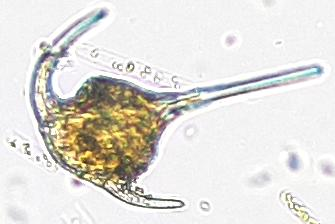
\includegraphics[width=\linewidth]{latex/figures/00_26_15_300342_10.jpg}
            \caption{\textit{Tripos} spp. (PlanktoScope)}
            \label{fig:tripos-ps}
        \end{subfigure} &
        \begin{subfigure}[b]{0.49\linewidth}
            \centering
            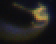
\includegraphics[width=\linewidth]{latex/figures/20231003_162111.225.0.png}
            \caption{\textit{Tripos} spp.\ \ \ \ \ \ \ \ \ \ \  (CPICS)}
            \label{fig:tripos-cpics}
        \end{subfigure} \\
        \begin{subfigure}[b]{0.49\linewidth}
            \centering
            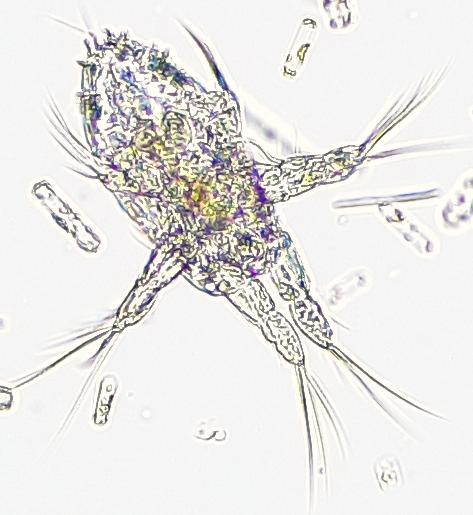
\includegraphics[width=\linewidth]{latex/figures/10_14_13_237354_14.jpg}
            \caption{Copepod naupli (PlanktoScope)}
            \label{fig:naupli-ps}
        \end{subfigure} &
        \begin{subfigure}[b]{0.49\linewidth}
            \centering
            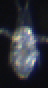
\includegraphics[height=\linewidth, angle=90,origin=c]{latex/figures/20230925_115158.468.0.png}
            \caption{Copepod naupli \ \ \ \ \ \ \ \ \ \ \  (CPICS)}
            \label{fig:naupli-cpics}
        \end{subfigure}
    \end{tabular}
    \caption{Examples and comparison of images from the PlanktoScope and CPICS. PlanktoScope images (a, c) have high resolution for small organisms and a light background. CPICS images (b, d) have lower resolution, but the throughput of the method is higher.}
    \label{fig:plankton-img}
\end{figure}

Samples for the PlanktoScope were taken with a plankton net from the shore in Drøbak, the Oslofjord, Norway (59.6635 N, 10.6256 E). The samples were pre-filtered through a 200 µm mesh sieve, and run through the PlanktoScope. The CPICS was deployed from a pier in Drøbak in October 2023. Both imagers have a built-in segmentation and feature extraction, which isolate regions of interest from the images and create metadata with, e.g., the size and shape of objects. The segmented images were manually classified in the Ecotaxa web portal (\hyperlink{https://ecotaxa.obs-vlfr.fr/}{https://ecotaxa.obs-vlfr.fr/}).

Ecotaxa has its own built-in classifier that you can train on your own data after manually labeling parts of the data. This is based on a random forest [REF], and by default uses a selection of the extracted metadata as input features. However, Ecotaxa also supports using what they call "deep features" for classification, which are features extracted from the images with using a CNN and then a dimensionality reduction method \footnote{see https://github.com/ecotaxa/ecotaxa_ML_template/tree/main}. Some of the labels for our images were created with this classifier, but most were validated by a human afterwards.

For the PlanktoScope images, we used a small validated subset consisting of 2,061 images with 14 different categories. The categories were slightly imbalanced, with most consisting of 200 images, but some with as little as 59. For the CPICS, we used all the validated data from the deployment, amounting to 222,000 images with 81 different categories. This data set was very imbalanced, with numbers in the categories ranging from 1 to 60,000. The ML methods we use here will be affected by this imbalance, and we expect them to perform poorly especially for the low-abundance categories. However, from a practical usage perspective it is important to keep rare categories, as these will show up in natural data sets.

\subsubsection{Image preprocessing}

The segmentation process in both imagers result in images of different dimensions, depending on the size and shape of the imaged object. However, most deep learning image classification methods require input images to be square with a specific resolution (REF). A common strategy is simply to reshape and resize the image to the right dimensions (REF), but this distorts the original shape of the object of interest, which could be important for correctly classifying plankton (REF?). Instead, we opted to resize only the largest dimension of the image to the correct resolution, and then pad the smallest dimension with the median edge color of the image. Since the images have an uniform light or dark background, the padding does not have a visible border, and should affect the classification minimally.

% =========================================================================
\subsection{Decision Trees}\label{ssec:decision_trees}
As the name suggests, decision trees are based on a tree structure, and the most popular method is the classification and regression (CART) algorithm. These models are often used for classification tasks as they are easy to visualize and interpret, allowing a clear understanding of how the model came to a decision. A tree consists of one root node, multiple internal nodes and leaf nodes, all connected by branches, as seen in Figure \ref{fig:decision_tree}. 
\begin{figure}[h!]
    \centering
    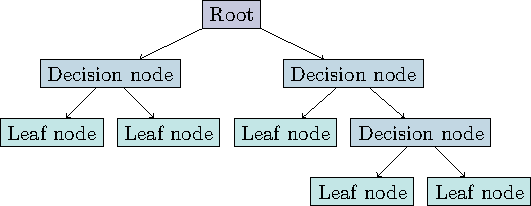
\includegraphics[width=0.9\linewidth]{latex/figures/dtree.pdf}
    \caption{Illustration of a decision tree, with a root node, three internal nodes referred to as decision nodes, and five leaf nodes.}
    \label{fig:decision_tree}
\end{figure}
The algorithm is based on finding the features in the data that best predict the target. The features that contain the most information about the target are referred to as informative, whereas those that do not are referred to as impure. To grow a tree the data is split according to a given criterion, where the aim is to find the most pure subset of data. This results in leaf nodes that correspond to predictive regions. Three common criteria for the best split in decision trees are entropy, the Gini index, and misclassification error.

\subsubsection{Split critera}\label{sssec:splitting_criteria}
The proportion of target class $k = 1, 2, \dots, K$ observations in a node $m$, defined for a region $R_{m}$ with $N_{m}$ observations, is defined as
\begin{equation}\label{eq:pdf_tree}
    p_{mk} = \frac{1}{N_{m}} \sum_{x_{i} \in R_{m}} I(y_{i} = k) .
\end{equation}
The proportion $I(y_{i} = k)$ represents the likelihood function used to determine the split of the data. This probability density function (PDF) is used in the following criteria. Entropy, or information entropy, is a measure of impurity and is defined as
\begin{equation}\label{eq:entropy}
    s = - \sum_{k=1}^{K} p_{mk} \log p_{mk} ,
\end{equation}
in the range $[0, 1]$, where $0$ represents pure data. The Gini index, also known as the Gini impurity measure, is defined as 
\begin{equation}\label{eq:gini_index}
    g = \sum_{i=1}^{K} p_{mi}(1 - p_{mi}) ,
\end{equation}
in the range $[0, 1]$, where $0$ represents pure data. The misclassification error is defined as
\begin{equation}\label{eq:misc_error}
    err = \frac{1}{N_{m}} \sum_{x_{i} \in R_{m}} I(y_{i} \neq k) = 1 - p_{mk},
\end{equation}
The different criterias can all be used, but some situations may favor one criteria over the others. In situations where the classification problem is binary, the Gini index is often preferred due to computational efficiency. Whereas entropy is preferred when the data is imbalanced, as it is a measure of the information needed to describe nodes of a given purity \cite[p. 309]{hastie:2009:elements}.

\subsubsection{The CART algorithm}\label{sssec:cart_algorithm}
The CART algorithm determines the data split using a feature and threshold pair, then minimizes the cost function
\begin{equation}\label{eq:cost_cart}
    C(k, t_{t}) = \frac{m_{left}}{m} g_{left} + \frac{m_{right}}{m} g_{right} , 
\end{equation}
here using the Gini index $g$. The tree is grown by recursively split into subsets and evaluating the cost function at each step. This is a greedy method, as it evaluate all possible splits at each step in building the tree. It does, however, not look ahead and only considers the current best split. In addition, if no stopping condition is given, the tree is prone to overfitting. 

\subsubsection{Pruning}\label{sssec:pruning}
One way to prevent overfitting is to prune the tree to obtain a smaller tree, which generalizes better to unseen data. The pruning can be performed by growing a tree $T_{0}$ to a given size (pre-pruning), then determine the trade-off between complexity and fit. A post-pruning method is known as cost complexity pruning, is applied on a fully grown tree. For this method idea is to find a sub-tree $T_{\alpha} \subseteq T_{0}$ for each value of the regularization parameter $\alpha$ to minimize 
\begin{equation}
    C_{\alpha} (T) = \sum_{m=1}^{|T|} N_{m} Q_{m}(T) + \alpha |T| .
\end{equation}
The number of terminal nodes in $T$ is denoted by $|T|$, and 
\begin{equation}
    Q_{m} (T) = \frac{1}{N_{m}}\sum_{x_{i} \in R_{m}} (y_{i} - \overline{y}_{R_{m}})^{2}  
\end{equation}
is a measure of the node training error. By collapsing a number of internal nodes until only the root node remains, a sequence of sub-trees is obtained for which we can find the optimal tree $T_{\alpha}$ \cite[p. 308]{hastie:2009:elements}. Cross-validation can be used to find the optimal parameter $\hat{\alpha}$, particularly if data is limited. Decision trees are, however, sensitive to small changes in the data, a limitation which can be improved by boosting methods such as AdaBoost.

\subsection{AdaBoost}\label{ssec:adaboost}
Boosting methods combine the output of several "weak" classifiers, where the error rate is slightly better than random guessing, to produce a good classifier. A popular method is AdaBoost, an adaptive boosting method, where a weak classification method is applied iteratively to repeatedly modified versions of the data, to produce a sequence of weak classifiers $G_{m}(x)$ \cite[p. 337]{hastie:2009:elements}. The error is  the weighted misclassification error in Equation \eqref{eq:misc_error}, and defined as
\begin{equation}
    \overline{err}_{m} = \frac{\sum_{i=0}^{n-1} w_{i}^{m} I(y_{i} \neq G(x_{i})}{\sum_{i=0}^{n-1} w_{i}} ,
\end{equation}
where the weights $w$ are initialize uniformly such that  $\sum_{i=0}^{n-1} w_{i} = 1$. For each iteration $m = 1, 2, \dots, M$ the error is computed and the weights are updated according to 
\begin{equation}
    w_{i} = w_{i} \times \exp (\alpha_{m} I(y_{i} \neq G(x_{i})))
\end{equation}
where $\alpha_{m}$ is defined as 
\begin{equation}
    \alpha_{m} = \frac{\log (1 - \overline{err}_{m})}{\overline{err}_{m}} .
\end{equation}
A new classifier is computed for each iteration, and the final prediction is given by 
\begin{equation}
    G(x) = sign \bigg( \sum_{m=1}^{M} \alpha_{m} G_{m}(x) \bigg) ,
\end{equation}
which is a weighted majority vote of the weak classifiers. We used decision trees as weak classifiers. 

% To do: gridsearch setup for both decision tree and adaboost, as part of method and/or result?

\subsection{Convolutional neural networks}

Fully-connected feed-forward neural networks (FCNN) can be used for a variety of tasks, including image recognition. However, these require flattening of the input data, which means that you may lose important characteristics when working with images, such as the position of the pixel and the value of adjacent pixels. Instead, it is common to use convolutional neural networks (CNNs), which keep these features, for image classification tasks. In a CNN, you create a feature map from your image where each element is just connected to a small group of pixels, in contrast to a FCNN where all nodes are connected \cite{raschka:2022:ml_pytorch_scikit}.

CNNs are based on the mathematical concept of convolution, which combines two functions into a third through the operation
\begin{equation}
    y(t) = \left(x * w\right)(t) = \int x(a) w(t-a) da.
\end{equation}
We here describe convolution for 1-dimension, but the operation can be generalized to higher dimensionalities. The discrete case of the convolution operation for two input vectors (in the 1D-case) is
\begin{equation}
    y = x * w \rightarrow y_i = \sum_{k=-\infty}^{\infty} x[i-k]w[k],
\end{equation}
and is commonly used for machine learning applications \cite{raschka:2022:ml_pytorch_scikit}. In practice, it is common to constrain the operation to the limits of the input data, i.e., rather than summing over infinite values you define the operation as
\begin{equation}
    y = x * w \rightarrow y_i = \sum_{k=0}^{k=m-1} x[i+m-k]w[k].
\end{equation}
For this operation, some indices fall outside of the ranges of the data. It is then common to pad the input vectors with zeros to still be able to compute the sums \cite{raschka:2022:ml_pytorch_scikit}.

Convolution can also be visualized as a filter vector moving across another, longer, vector and calculating the dot product of the overlapping elements (see, e.g., \cite{raschka:2022:ml_pytorch_scikit} p.456 fig. 14.3). The filter has to be rotated in all dimensions before being compared with the vector to align with the mathemathics of convolution. A related method to convolution is cross-correlation, defined as
\begin{equation}
    y = x \star y = \rightarrow y_i = \sum_{k=-\infty}^{\infty} x[i+k]w[k].
\end{equation}
In many machine learning applications, cross-correlation is used instead of convolution but is still commonly referred to as convolution \cite{raschka:2022:ml_pytorch_scikit}.

A CNN consists of several types of layers, most often a series of convolutional and pooling layers followed by one or more fully-connected layers. In a convolutional layer, a $n \times n$ filter with weights applies a convolution (or cross-correlation) operation to the input data, reducing the size of the original image. This process can be visualized as the filter "moving across" the image, calculating a weighed sum of a (for a 2D greyscale image) $n \times n$ subset of pixels, before moving to the next subset of pixels with step size (stride) $S$ (with or without overlap, depending on $n$ and $S$) \cite{dumoulin2016guide}. In this process, the center pixels are included in several of the summations, while the corners only get used once. To avoid overemphasizing the center pixels compared to the edges, it is common to pad the input data with zeros at the ends, where the number of padding values are specified with the parameter $p$ \cite{raschka:2022:ml_pytorch_scikit}. The size of the filter $n$, stride $S$ and padding $p$ are all hyperparameters of the model that can be tuned.

After a convolution step, the output is transformed with an activation function, commonly the ReLU function
\begin{equation}
    \text{ReLU(x)} = \max(0,x).
\end{equation}
The dimensionality of the output of the activation is then further reduced by pooling. The pooling takes subsets of the data (without overlap) and reduces it to a single value either by using the maximum value (max pooling) or mean (average pooling) of the subset. The ReLU and pooling functions have no trainable parameters.

It is common to apply several steps of convolution, ReLU and pooling. After this, the output is flattened to 1 dimension and used as input a FCNN. For classification, the output layer of the FCNN commonly uses softmax activation
\begin{equation}
\label{eq:softmax}
\text{Softmax}(\mathbf{x_i}) = \frac{e^{x_i}}{\sum_{j} e^{x_j}},
\end{equation}
and has the same size as the number of categories. Like in a regular FCNN, it is common to use the cross-entropy loss function

INSERT CROSS-ENTROPY EQ HERE,

and it is also possible to include (for example) L2 regularization

L2 REGULARIZATION

to avoid overfitting

Training CNNs can be time-consuming and require extensive data (REF). An alternative is 

% EB writes here - this is method but parts of it can also be included in introduction.

\subsection{Vision Transformers} \label{ssec:vit}

\subsubsection{Transformers and the self-attention mechanism}
Vision transformers are based on transformers, but applied to images (introduction). For a transformer with text inputs, each word in the text are considered tokens. When fed into the model, each token produces its own embedding vector in space, $\vec{E}_i$ for $i = {1, 2, ..., n}$. Then, key $\vec{K}_i$ and query $\vec{Q}_i$ vectors are found using weight parameters for each vector
\begin{equation}
    \begin{split}
    \vec{Q}_i = \boldsymbol{W_Q} \vec{E}_i  \\
    \vec{K}_i = \boldsymbol{W_K} \vec{E}_i . \\
    \end{split}
\end{equation}
Each of these vectors combined make out the key and query matrices $\boldsymbol{K}$ and $\boldsymbol{Q}$. If we find
\begin{equation}
    Attention\ map = \boldsymbol{QK^T},
\end{equation}
this attention map tells us which embeddings attend to each other - or said differently, which tokens that are likely to be in the same context. The attention map as it's shown here is simply an $n x n$ matrix that describe how tokens relate to each other by the size of the computed dot product between 
\begin{equation}
   A_{i, j} =  \boldsymbol{W_Q} \vec{E}_i \ \cdot \ \boldsymbol{W_K} \vec{E}_j, 
\end{equation}
where $A_{i, j}$ is an element in the attention map. 

The original authors refer to their attention mechanism as a "Scaled Dot-Product Attention", which they present mathematically as
\begin{equation}
    Attention(\boldsymbol{Q, K, V}) = \frac{\boldsymbol{QK^T} V}{\sqrt{d_K}}.
\end{equation}
The $d_K$ represents the dimension for matrix $\boldsymbol{K}$ (which is equal to the dimension of $\boldsymbol{Q}$), and the scalar $\frac{1}{\sqrt{d_K}}$ constitutes the "scaled" part of the "Scaled Dot-Product Attention", and authors state it was added for numerial stability. This new matrix $\boldsymbol{V}$ is a concatenation of a set of value vectors $\vec{V}_i = \boldsymbol{W_V}\vec{E}_i$. If we then find
\begin{equation}
    \Delta\vec{E}_i = \vec{V}_i A_j  
\end{equation}
for all combinations of $i$ and $j$ so that each value vector is multiplied with each column of the attention map, the resulting term $\Delta\vec{E}_i$ is what we use to update the embedding of the original token so that $\vec{E}_i  = \Delta\vec{E}_i + \vec{E}_i $. 

During training of a transformer, all the weight matrices $\boldsymbol{W_K, W_Q , W_V}$ get continuously updated so that the embeddings are shaped into more contextualized tokens. Most attention heads then feed their updated embeddings into an MLP network for later classification. 

This description of the transformer self-attention mechanism has skipped a few steps such as the masking of the attention map as well as the positional embedding process. Here we have outlined the very distinct functionality for a single transformer attention head, however, most transformers have several attention heads performing this computation in parallel. 

\subsubsection{Vision transformers}

A vision transformer (ViT) splits an image into even sized, non-overlapping patches, which are then linearly embedded
as token representations. These tokens are then fed into the regular transformer architecture. The previously mentioned attention mechanism is then used during training
so that the model considered spatial relationships within and between patches. The original layout of a ViT is presented in Figure \ref{fig:ViT}.

% The authors of this 
% report will not pretend to understand the ViT completely, but we provide the reader with all sources
% to fully comprehend this architecture, and present the original layout of a ViT in Figure \ref{fig:ViT}

\begin{figure}[H]
    \centering
    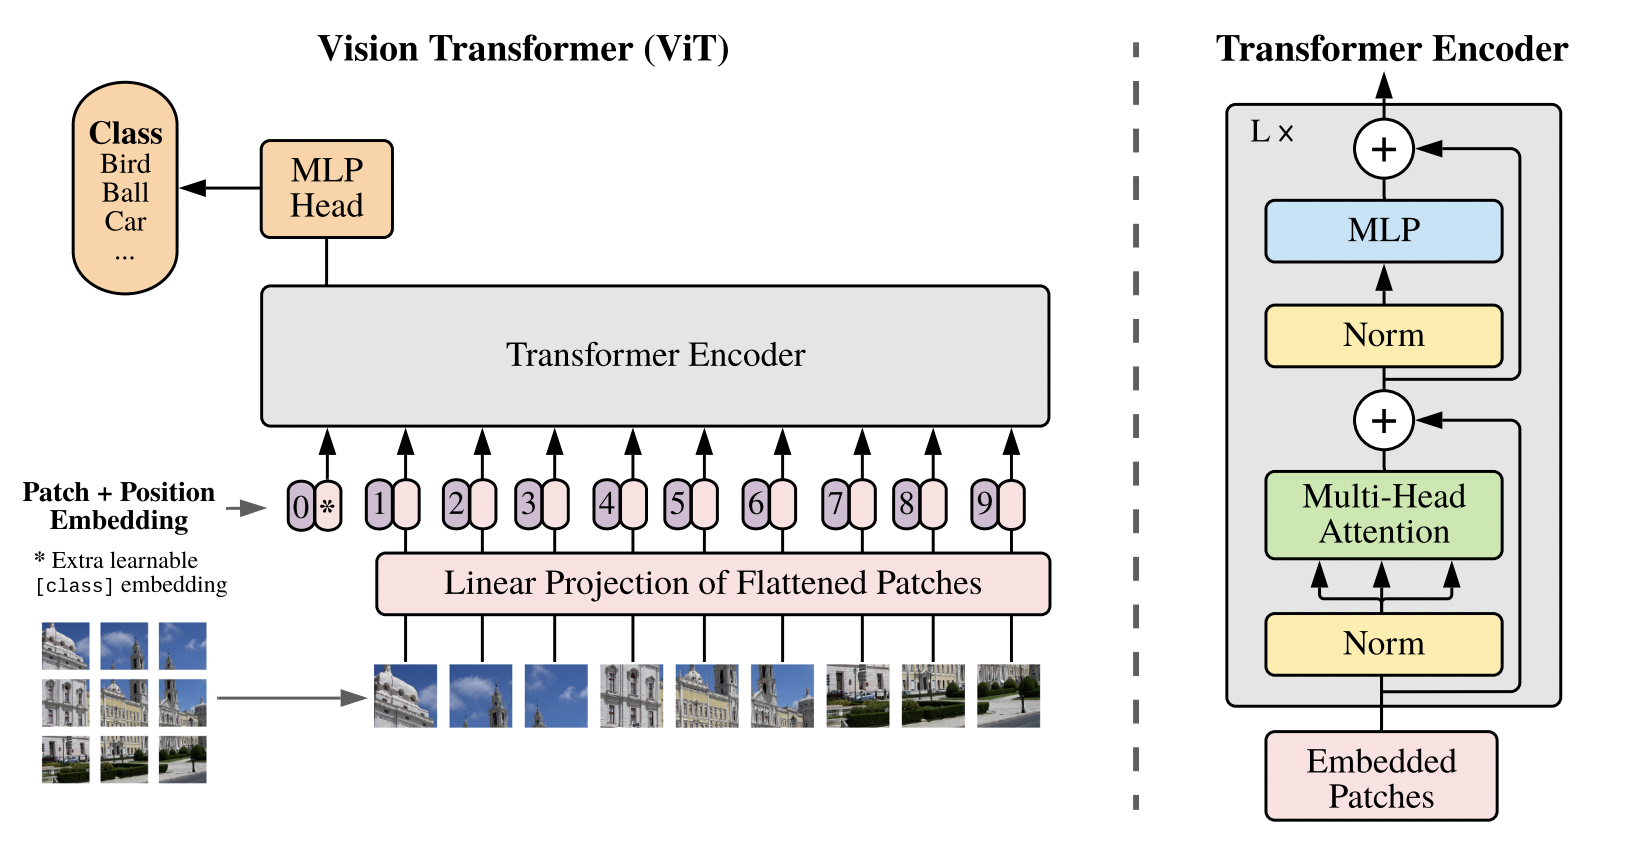
\includegraphics[width=1\linewidth]{examples/tests_eb/figs/vit.png}
    \caption{Vision Transformer layout as presented from it's original paper by Dosovitskiy et. al \cite{first_vit}. The Multi-Head attention layer is what we've previously described as a self-attention layer. The MLP layer stands for Multi Layer Perceptron, this is the same as a multi-layer FCNN.}
    \label{fig:ViT}
\end{figure}

\subsubsection{Self-\textbf{di}stillation with \textbf{no} labels (Meta's \textbf{DINO})} \label{sssec:dino}

In DINO, the self-\textbf{di}stillation aspect refers to a teacher-student interaction, where a teacher model looks into global augmented crops of an image and the student model looks into both smaller (local), augmented crops and global, augmented crops of the same image patch. The goal is that both the student and the teacher gives us the same feature representation of the different crops, essentially teaching the model that minor deviations in size and color should still fall into the same representation. 

During training, the weight matrices of the student model are updated to minimize the loss, while the teacher’s parameters are updated using an exponential moving average (ema) of the student’s weights. A simple figure that aims to illustrate this is shown in Figure \ref{fig:dino}, and an even better gif illustrates this on DINO's \hyperlink{https://github.com/facebookresearch/dino}{Github}.

%
The DINO loss function formalizes this teacher-student relationship mathematically. For both the teacher and student models, respective feature vectors derived from the same image patch, but with a different set of augmentations $x_1 \text{ and } x_2$ are extracted from the token of a ViT. These vectors are passed through the MLP to produce prototype scores, which are then turned into probabilities using the softmax function from Eq. (\ref{eq:softmax}), more specifically

\begin{equation} \label{eq:dino-softmax}
p_1(x)^{(i)} = \frac{\exp\left(g_{\theta_s}(x)^{(i)} / \tau_s\right)}{\sum_{k=1}^K \exp\left(g_{\theta_s}(x)^{(k)} / \tau_s\right)},
\end{equation}
where $\tau$ is a temperature parameter that performs the sharpening of the signal. It leads to an exaggeration of small differences in the distribution, meaning peaks become more pronounced. The $\theta$ for student and teacher represent the parameters in the architecture, while $g_\theta$ represent the shared architecture of the student and teacher, this can either be CNN or ViT.

We call the student probabilities \( p_1 \) and the teacher probabilities \( p_2 \). The loss function is then defined as
\[
\mathcal{L}_{\text{DINO}} = -\sum p_2 \log p_1,
\]
and minimized using using stochastic gradient descent. Similarly, the teacher’s embedding vectors are processed to generate its prototype scores, which are centered using an exponential moving average 
\begin{equation} \label{eq:ema}
\theta_t \gets \lambda \theta_t + (1 - \lambda) \theta_s. 
\end{equation}
%
The decay factor $\lambda$ is following a cosine schedule from 0.996 to 1 during training. This equation represents how the teacher is updated with a momentum average, which also means that it is considered a momentum teacher.

Finally, centering of the teacher output can be written as so
\begin{equation}
c \gets mc + (1 - m) \frac{1}{B} \sum_{i=1}^B g_{\theta_t}(x_i),
\end{equation}
where $m > 0$ is a rate parameter and $B$ is the batch size. The authors intorduce this as a way to balance out the sharpening effect taking place in Eq. (\ref{eq:dino-softmax}) on the distribution output of the softmax function, as the centering pushes the distribution towards more a uniform shape while the sharpening has the opposite effect.
%
%
%
\begin{figure}[H]
    \centering
    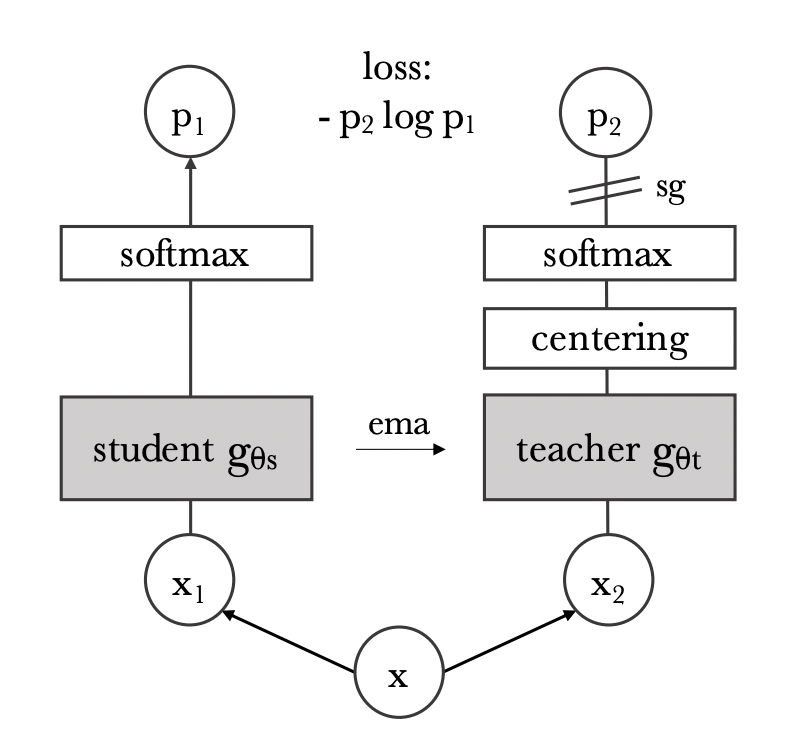
\includegraphics[width=0.7\linewidth]{examples/tests_eb/figs/dino.png}
    \caption{Student-Teacher interactions as presented in original DINO article \cite{dino1} for a single token. The gray boxes with $g\theta$ represent the shared architecture of the student and teacher. The ema function is an exponential moving average. The sg is a stop-gradient operator that ensures gradients are propagated only through the student.}
    \label{fig:dino}
\end{figure}
%
%


The original DINO's performance has improved with Meta's newest release of the updated \textbf{DINOv2} \cite{dino2} from january 2024. the model produces a set of 384 embeddings and has been trained on LVD-142M, meaning 142 million images. The authors themselves make the claim that the newest DINOv2 does not require any fine tuning, and we've therefore chosen to go for their reccomended approach. 

\begin{table}[H]
\centering
\caption{ViT architecture details for DINOv2 ViT-S}
\begin{tabular}{c|c}
\textbf{ViT Model} & DINOv2 ViT-S \\ \hline
Params & 21M params \\ 
Patch Size & 14 \\ 
Embedding Dimension & 384 \\
Attention heads & 6 \\ 
NN Architecture & MLP FFN \\
Training Data & LVD-142M \\ 
\end{tabular} \label{tab:vit-params}
\end{table}

We present the architecture of our chosen DINOv2 in Table \ref{tab:vit-params}. This is the same for student and teacher, but in the end it is the teacher parameters that we import to extract our feature embeddings. We went with one of their smaller models for this project, even though it has worse performance, in order to save some time when running the large data set. Their current best DINOv2 model is the ViT-g with 1.1B params, but this we save for later use.



\subsection{Dimensionality Reduction and Clustering}
We reduce the dimensionality of our ViT-derived feature and perform simple clustering methods on the reduced features. Our methods include Prinipal Component Analysis, Uniform Manifold Approximation and Projection for
Dimension Reduction and K-means clustering. 

\subsubsection{Principal Component Analysis (PCA)}
Consider a classic design matrix
$$
\boldsymbol{X}=\begin{bmatrix}
x_{0,0} & x_{0,1} & x_{0,2}& \dots & \dots x_{0,p-1}\\
x_{1,0} & x_{1,1} & x_{1,2}& \dots & \dots x_{1,p-1}\\
x_{2,0} & x_{2,1} & x_{2,2}& \dots & \dots x_{2,p-1}\\
\dots & \dots & \dots & \dots \dots & \dots \\
x_{n-2,0} & x_{n-2,1} & x_{n-2,2}& \dots & \dots x_{n-2,p-1}\\
x_{n-1,0} & x_{n-1,1} & x_{n-1,2}& \dots & \dots x_{n-1,p-1}\\
\end{bmatrix},
$$
where the rows $n$ represent our data points, or images, while the columns $p$ represent our features. This can be written as 
$$
\boldsymbol{X}=\begin{bmatrix} \boldsymbol{x}_0 & \boldsymbol{x}_1 & \boldsymbol{x}_2 & \dots & \dots & \boldsymbol{x}_{p-1}\end{bmatrix}.
$$
Here, each vector $\mathbf{x_i}$ for $i = [0, 1, \cdots, p-1]$ represents a feature, and all of the elements contained in the vector represent how a single data-point is described by that feature. If we then observe a mean centered covariance matrix written as 
$$
\boldsymbol{C}[\boldsymbol{x}] = \begin{bmatrix}
\mathrm{var}[\boldsymbol{x}_0] & \mathrm{cov}[\boldsymbol{x}_0,\boldsymbol{x}_1]  & \dots  & \mathrm{cov}[\boldsymbol{x}_0,\boldsymbol{x}_{p-1}]\\
\mathrm{cov}[\boldsymbol{x}_1,\boldsymbol{x}_0] & \mathrm{var}[\boldsymbol{x}_1]& \dots & \mathrm{cov}[\boldsymbol{x}_1,\boldsymbol{x}_{p-1}]\\
\mathrm{cov}[\boldsymbol{x}_2,\boldsymbol{x}_0]   & \mathrm{cov}[\boldsymbol{x}_2,\boldsymbol{x}_1] & \dots  & \mathrm{cov}[\boldsymbol{x}_2,\boldsymbol{x}_{p-1}]\\
\dots & \dots & \dots & \dots & \\
\mathrm{cov}[\boldsymbol{x}_{p-1},\boldsymbol{x}_0]   & \mathrm{cov}[\boldsymbol{x}_{p-1},\boldsymbol{x}_1]  & \dots  & \mathrm{var}[\boldsymbol{x}_{p-1}]\\
\end{bmatrix},
$$
we can re-write this as 
$$
\boldsymbol{C}[\boldsymbol{x}] = \frac{1}{n}\boldsymbol{X}^T\boldsymbol{X}= \mathbb{E}[\boldsymbol{X}^T\boldsymbol{X}]
$$
by the classic definition of the covariance matrix. We then move into the spectral theorem, where $\boldsymbol{A} = \boldsymbol{SDS^{-1} = SD S^T}$, and $\boldsymbol{S}$ is some orthogonal matrix. Then:
\begin{equation}
\begin{split}
    \boldsymbol{A^T} & = \boldsymbol{(S D S^T)^{T}} \\ 
    & = \boldsymbol{ (S^T)^T D^T S^T =  S D S^T = A}.
\end{split}
\end{equation}
Here, $\boldsymbol{A}$ is a symmetric matrix where there exists a basis for each finite dimensional vector space, and $\boldsymbol{D}$ is a diagonal matrix with the eigenvalues of $\boldsymbol{A}$ as it's signature. 
\\
\\
If we assume there exists a transformation $\boldsymbol{S}^T\boldsymbol{C}[\boldsymbol{x}]\boldsymbol{S}=\boldsymbol{C}[\boldsymbol{y}]$ so that the resulting matrix $\boldsymbol{C}[\boldsymbol{y}]$ is a diagonal matrix with the signature $\vec{\lambda}= [\lambda_0,\lambda_1,\lambda_2,\dots,\lambda_{p-1}]$, 
we can derive the following expression
\begin{equation}
\begin{split}
\boldsymbol{C}[\boldsymbol{y}] = \boldsymbol{S}^T\boldsymbol{C}[\boldsymbol{x}]\boldsymbol{S}. \\
\end{split}
\end{equation}
If we multiply the matrix $\boldsymbol{S}$ from the left on either side and consider that our matrix $\boldsymbol{C}[\boldsymbol{y}]$ is in fact a diagonal matrix written as $\boldsymbol{C}[\boldsymbol{y}], = \boldsymbol{I}\vec{\lambda} = \boldsymbol{\lambda }$, we're left with the expression
\begin{equation}
\begin{split}
\boldsymbol{S}\boldsymbol{C}[\boldsymbol{y}] & = \boldsymbol{C}[\boldsymbol{x}]\boldsymbol{S} \\
\boldsymbol{S} \boldsymbol{\lambda}\boldsymbol{S^T} & = \boldsymbol{C}[\boldsymbol{x}].
\end{split}
\end{equation}
% Consider putting all the math in appendix, tmi! 
\\
\\
When solving for a set of principal components, we wish to find the eigenvalues and eigenvectors of our covariance matrix $\boldsymbol{C[x]}$, where one principal component is an eigenvector $\vec{v_i}$ and the importance (or variance expained) by said vector is determined by the corresponding eigenvalue $\lambda_i$. This is then the same as solving the above equations for $\boldsymbol{\lambda}$ and $\boldsymbol{S}$, as the columns $\vec{s}_i$ in the latter are the corresponding eigenvectors to $\lambda_i$. Thus we're solving a set of equations

\begin{equation}
    \boldsymbol{C[x]} \vec{s}_i= \lambda_i\vec{s}_i.
\end{equation}
%
This is done through Single Value Decomposition (SVD) through existing libraries as we describle in our Tools section \ref{subsec:tools}. When discussing PCA, it is also important to introduce the term explained variance ratio, as we use this to illustrate the variance contribution from each eigenvector. The cumulative variance for a subset of eigenvalues $r+1$ from a total set of $n+1$ is written as
\begin{equation}
    cum\ variance(\lambda_0, \cdots, \lambda_r)  = \frac{\sum_{i = 0}^{i = r} \lambda_i}{\sum_{i = 0}^{i = n-1} \lambda_i}
\end{equation}



\subsubsection{Uniform Manifold Approximation and Projection for Dimension Reduction (UMAP)}
UMAP is a newer dimensionality reduction technique presented by Leland et. al 2020 \cite{umap}. The authors describe it as a cross-entropy minimization problem where a low-dimension topographical representation of the data $Y$ is altered to approximate a high-dimensional topographical dimension $X$.

In simple terms, the method first construct a set of fuzzy set approximations for both Y and X. A fuzzy set of $i$ enumerated elements from a carrier set $A$ has a map, or a membership function $u : A \rightarrow I$ where $u(x) \in [0, 1]$. This can also be interpreted as the degree of truth to the sentence "$x$ belongs to $A$". In cases where $u(x) \in \{0, 1\}$, we have a crisp set, while a fuzzy set can be written as $(A, u(x))$. 

UMAP is often presented as similar to t-SNE, as the dimensionality reduced embedding is optimized in a with respect to the fuzzy set cross entropy
\begin{equation}
\begin{split}
& \\
&C\left((A, \mu), (A, \nu)\right) \triangleq \\
&\sum_{a \in A} \left(\mu(a) \log \frac{\mu(a)}{\nu(a)} + (1 - \mu(a)) \log \frac{1 - \mu(a)}{1 - \nu(a)}\right).
\end{split}
\end{equation}
$(A, \mu)$ and $(A, \nu)$ are comparable fuzzy sets with different membership functions $\mu$ and $\nu$, taking in the enumerated elements $x$ from the original, shared carrier set $A$. The variable $a$ here is derived from the variable $x$, but we will not go into details on this. 

The fuzzy sets are then constructed as simpleces. A simplex is a way to build a $k$-dimensional object as illustrated in Figure \ref{fig:simpleces}. This combination results in what the authors refer to as "local fuzzy simplicial set representations". Finally, these representations are patched together to construct topographical representations of higher dimensional data. 

\begin{figure}[H]
    \centering
    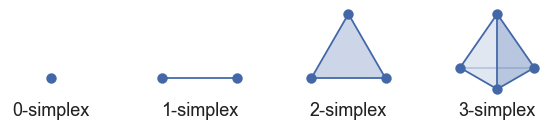
\includegraphics[width=1\linewidth]{examples/tests_eb/figs/Skjermbilde 2024-12-05 kl. 16.56.40.png}
    \caption{Simpeces illustrated here can be used to as combinatorial building blocks.}
    \label{fig:simpleces}
\end{figure}

One important thing to note about the UMAP is that it is optimized by stochastic gradient descent, and therefore clustering results are not reproducible. To work around this, we implemented the method with a set seed, even though the authors warn that might cause a slight reduction in performance. 

The full paper on UMAP is around 60 pages long, and we will not deny that the concepts of manifold approximations are a bit too advanced for us to do by hand. Luckily, UMAP is available as a package in Python and very user friendly. We expect the UMAP dimensionality reduction to capture a broader spectrum of variance and therefore include this as one of our unsupervised methods.

\subsection{Tools} \label{subsec:tools}
The decision tree and Adaboost methods were implemented using \verb|scikit-learn|. We used \verb|GridSearchCV|, provided by the same package, to find the optimal parameters for both models by parameter grid search.



%
% =========================================================================

% =========================================================================
%
% Janita writes here
%
% =========================================================================

% =========================================================================
%
% Even writes here
%
% =========================================================================